\subsection{ENI}

ENI rozwija specyfikacje w kierunku Kognitywnego Systemu Zarządzania, który będzie regulował działanie sieci poprzez wykorzystanie technik sztucznej inteligencji, takich jak \hyperlink{def:uczenie-maszynowe}{uczenie maszynowe (ang. \textit{machine learning})} oraz \hyperlink{def:wnioskowanie}{wnioskowanie (ang. \textit{reasoning})}. 

Z poprzedniej sekcji wiemy, że aby \hyperlink{def:wnioskowanie}{\textit{wnioskować}} potrzebna jest \hyperlink{def:wiedza}{\textit{wiedza}}. Skąd taki system pozyskiwałby wiedzę? Otóż, dzieje się to poprzez proces \hyperlink{def:uczenie-maszynowe}{\textit{Uczenia Maszynowego}}. Pierwsza faza czyli tzw. "trening", odbywa się jeszcze przed wdrożeniem systemu. Ale system również może uczyć się "z doświadczenia" (ang. \textit{experience}), kiedy już jest w pełni operacyjny. Stąd mówimy o empirycznej inteligencji sieciowej (ang. \textit{experiential networked intelligence}). 

Czyli z jednej strony \hyperlink{def:wiedza}{\textit{wiedza} potrzebna do \hyperlink{def:wnioskowanie}{wnioskowania,}} a w ostateczności podejmowania decyzji płynęłaby z samej sieci, co w przypadku telefonistki równoważne jest zapalającej się lampce na tablicy świetlnej. Z drugiej strony telefonistka ma również niejako wbudowaną w siebie wiedzę o tym, jak zorganizowane są łącza na przełącznicy komutacyjnej. Podobnie sieć musi mieć pewną części wiedzy nieco narzuconą z góry. Ta część wiedzy stanowi jako zestaw reguł używanych do zarządzania i kontrolowania stanu sieci. Takie reguły nazywamy \hyperlink{def:polityka}{\textit{politykami}}.

Polityki mogą płynąć od: aplikacji zarządzających siecią, użytkowników sieci, systemów OSS/BSS lub Orkiestratora. Ważne jest to, aby polityki były \hyperlink{def:swiadomosc-kontekstu}{\textit{świadome kontekstu}}. Pozwoli to na stworzenie systemu \hyperlink{def:kognitywnosc}{\textit{kognitywnego}}, czyli takiego, który uczy się, wnioskuje oraz podejmuje decyzje w sposób przypominający ludzki umysł. Taki system z kolei jest w stanie w dużym stopniu odciążyć operatora i zautomatyzować zadania jak: 

\begin{itemize}
    \item dynamiczne przydzielanie zasobów (ang. \textit{dynamic resource allocation}), 
    \item równoważenie obciążenia (ang. \textit{load balancing}), 
    \item zarządzanie wydajnością energetyczną (ang. \textit{energy efficiency management}, 
    \item samo naprawiające się sieci (ang. \textit{self-healing networks}), 
    \item optymalizacja jakości doświadczeń użytkowników (ang. \textit{QoE optimization}), 
    \item egzekwowanie polityk (ang. \textit{policy enforcement}), 
    \item zapewnienie zgodności z regulacjami (ang. \textit{regulatory compliance}) 
    \item i wiele innych.
\end{itemize}

\begin{figure}[!htbp]
    \centering 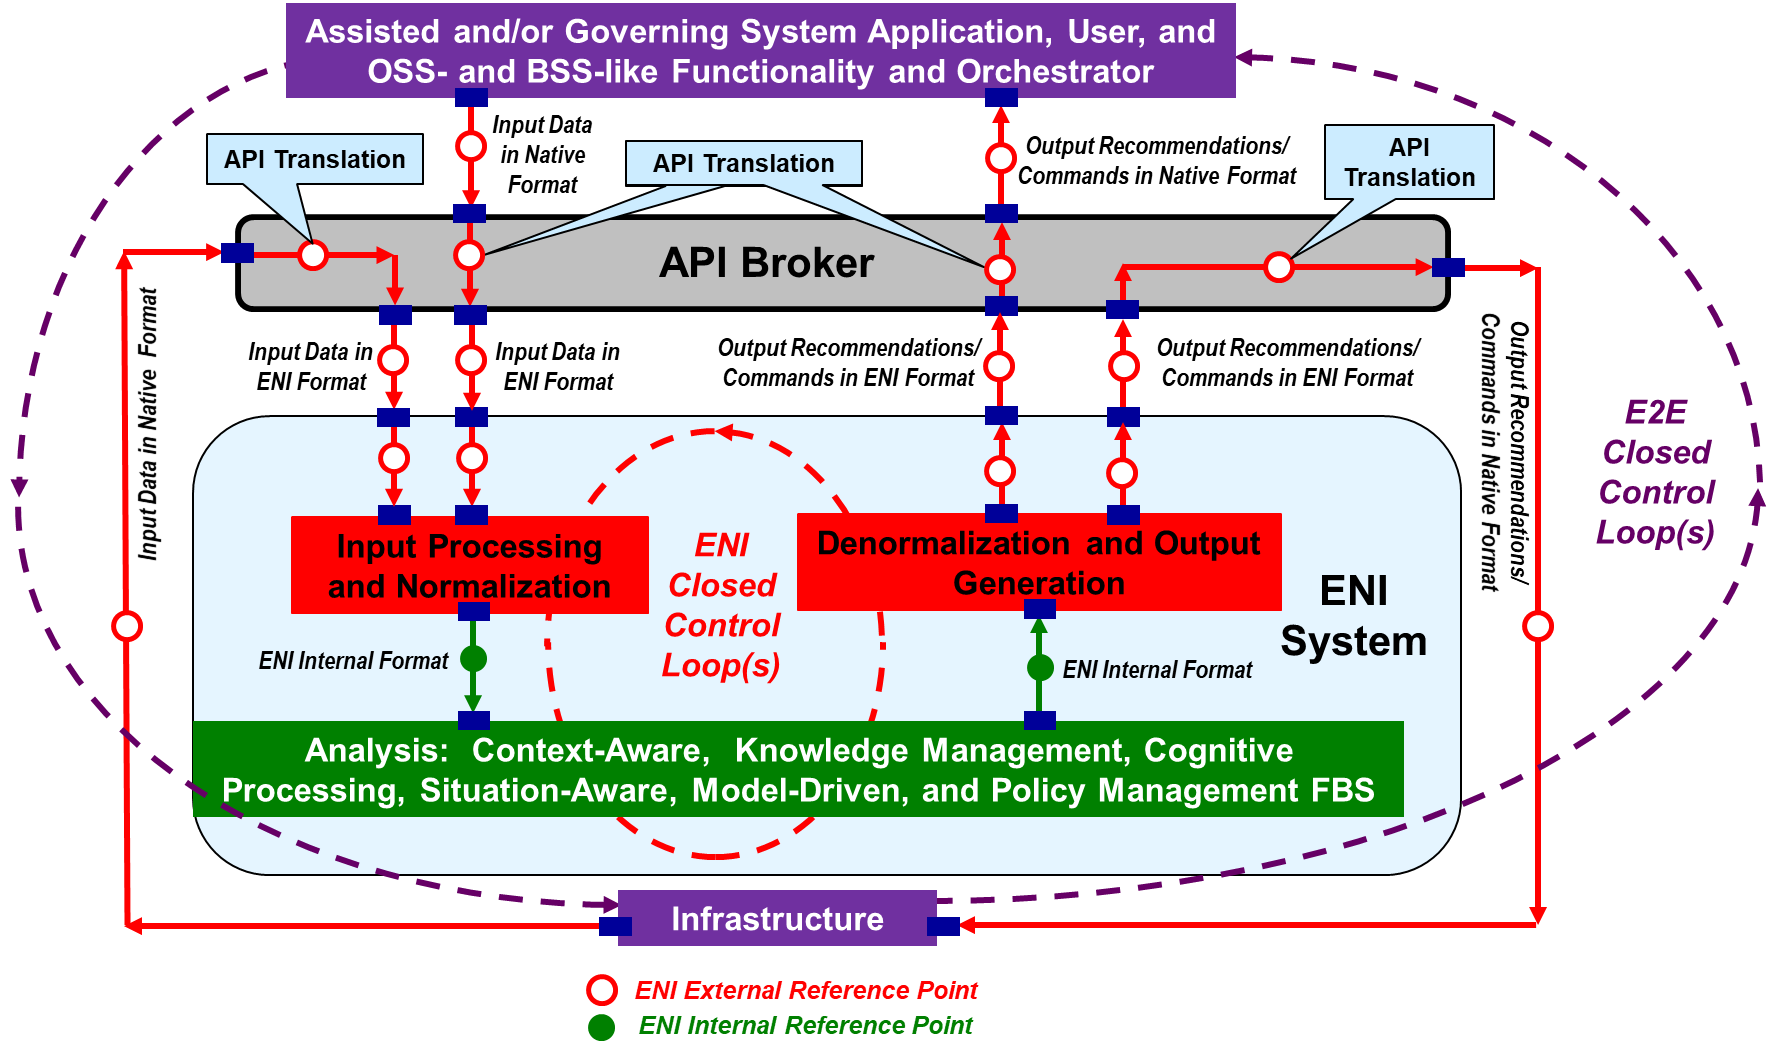
\includegraphics[width=1\linewidth]{23-eni-arch.png}
    \caption{Wysokopoziomowa architektura funkcjonalna ENI}\label{fig:23-eni-arch}
\end{figure}

Wysokopoziomową architekturę funkcjonalną ENI pokazano na rysunku \ref{fig:23-eni-arch}. Jej działanie można opisać jako dwie zamknięte pętle sterowania. Za pomocą zewnętrznej, system zarządzania (użytkownik, OSS/BSS, orkiestrator) reguluje pracę sieci (infrastruktury). Dokonuje tego nie bezpośrednio, lecz za pomocą \hyperlink{def:system-eni}{Systemu ENI}, który sam wewnętrznie również posiada zamkniętą pętle sterowania. Wewnętrzna pętla podczas wnioskowania bierze pod uwagę nie tylko wiedzę płynącą bezpośrednio z sieci, ale również tę od orkiestratora. Wszystkie komponenty odpowiedzialne za sztuczną inteligencję są umieszczone na rysunku \ref{fig:23-eni-arch} w zielonym prostokącie i stanowią \hyperlink{def:workflow}{\textit{workflow}} wewnętrznej pętli. 